\chapter[SCP-018 弹力球]{
    SCP-018 Super Ball\\
    SCP-018 弹力球
}

\label{chap:SCP-018}

\begin{figure}[H]
    \centering
    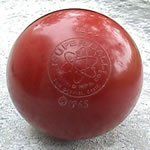
\includegraphics{images/SCP.018.jpg}
    \caption*{SCP-018}
\end{figure}

\bb{项目编号:}SCP-018

\bb{项目等级:}Euclid

\bb{特殊收容措施:}SCP-018须以长宽高均为1米的专用的密封金属箱收容,箱中填满高密度合成填料,并进一步浸在长宽高均为10米的聚乙烯存储罐的心部。若SCP-018脱离密封箱,以聚乙烯为基底的黏性物会削弱它的动能,以便管控人员回收。人员进入SCP-018的收容室须身着专用外覆金属甲(在SCP-018内部观察到该元素),下至聚乙烯存储罐前须戴防毒面具。若SCP-018脱离存储罐,建议现场人员进入别室以保证人身安全,并封锁走廊与舱门隔离该对象,等待管控小组到场。

\bb{描述:}表面上,SCP-018是一颗惠姆奥公司(Wham-O company)1969年产的弹力球(Super Ball),直径六公分,红色。██████████公司受雇清理一间曾存放惠姆奥公司的商品的仓库时发现了SCP-018异乎寻常的弹跳力。初看,SCP-018不过一件鲜艳的儿童玩具,但其弹跳效率超过了200\%(即,从1米高处落下,弹回2米,然后是4米,8米,16米)。小球马上变成了危险的炮弹,估计时速可达100公里以上。它在█████████████市毁坏了房屋并致五人受伤,几天后才停在附近的████████湖里,由SCP人员回收。鉴于对象的高速及受害者的猝不及防,无须编造事实掩盖真相。

\bb{文档018-04:}给O5-█的便条

\ii{█████████,一切安好?给你写信是因为,在回收新的或者逃跑的SCP对象方面,我已经发现了一个更有效的手段。我知道我在这玩意儿的逆向工程(reverse engineering)上毫无进展,天知道是什么鬼东西让它能违反热力学定律,但是我已经设法把它装在一具新型的SCP-A5装甲上了。听我说完,我们把它植入靴子底部,再安装点儿机械装置,锵锵,现在装甲可以轻松越过高楼大厦了。如果装甲的使用者想送什么东西下地狱,下个口令就能发出致命一踢。就是这种先期型的SCP-A5装甲,给我个改修许可,你就能确确实实地逮住████████████,再加上任何逃跑的SCP对象了。相信我,我什么时候让你失望了?}

——█████████博士

\bb{文档018-06:}致█████████博士的信

\ii{█████████博士:}

\ii{上次特工██████执行回收SCP-███的任务时,分配到了你的改良型SCP-A5装甲,但结果忧喜参半。好消息是,特工██████成功地给SCP-███套上了██████████项圈,在亚马逊好一通围追堵截,把它大卸八块才算控制住了局面。可是他现在折了两条腿、七根肋骨,一只胳膊没了,脑袋上还有一道大口子,就因为他回来时从一英里高的地方摔进了███████████湖里,就因为你那“小小的机械装置”出了点错儿。不把你的装甲修好就别想从我这儿得到投入使用的许可了。}

\bb{文档018-11:}给O5-█的便条

\ii{█████████,别担心,都搞定了。我有个主意,如果能让我用一用从\hyperref[chap:SCP-006]{SCP-006}打来的水、SCP-███甚至SCP-███的话,我就送你一套SCP-A5装甲外带一名特工,离群的野兽、没被确保的SCP,他们什么都抓得到,就等你一句话。}
